\documentclass[tikz,border=2pt]{standalone}
\usepackage{amsmath}
\begin{document}
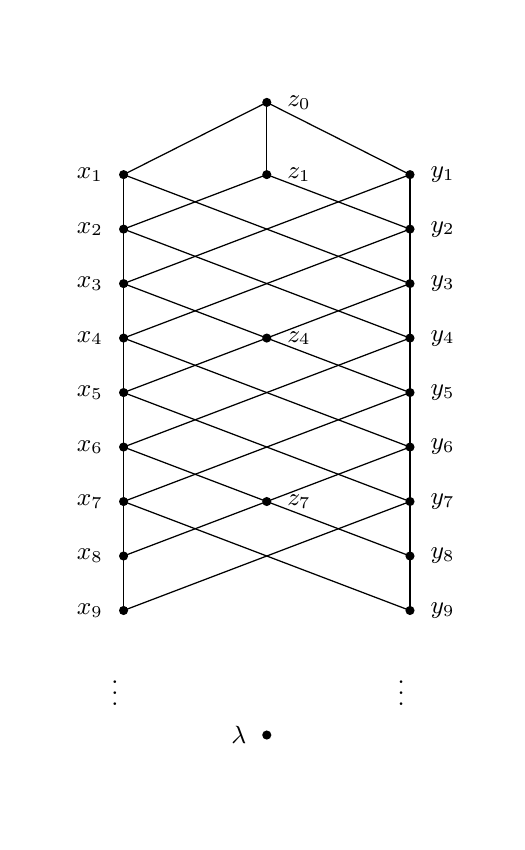
\begin{tikzpicture}[x=.45pt,y=-.45pt,line width=.45pt,line cap=round,font=\fontsize{9}{10}\selectfont]
\path[use as bounding box] (268,-18) rectangle (645,620);
\coordinate (ncap) at (460,42);
\coordinate (nx1) at (345,100);
\coordinate (ny1) at (575,100);
\coordinate (nx2) at (345,143.75);
\coordinate (ny2) at (575,143.75);
\coordinate (nx3) at (345,187.5);
\coordinate (ny3) at (575,187.5);
\coordinate (nx4) at (345,231.25);
\coordinate (ny4) at (575,231.25);
\coordinate (nx5) at (345,275);
\coordinate (ny5) at (575,275);
\coordinate (nx6) at (345,318.75);
\coordinate (ny6) at (575,318.75);
\coordinate (nx7) at (345,362.5);
\coordinate (ny7) at (575,362.5);
\coordinate (nx8) at (345,406.25);
\coordinate (ny8) at (575,406.25);
\coordinate (nx9) at (345,450);
\coordinate (ny9) at (575,450);
\coordinate (nz1) at (460,100);
\coordinate (nz4) at (460,231.25);
\coordinate (nz7) at (460,362.5);
\coordinate (ninfinity) at (460,550);
\draw (nx2) -- (nx1);
\draw (ny2) -- (ny1);
\draw (nx3) -- (nx2);
\draw (ny3) -- (ny2);
\draw (nx4) -- (nx3);
\draw (ny4) -- (ny3);
\draw (nx5) -- (nx4);
\draw (ny5) -- (ny4);
\draw (nx6) -- (nx5);
\draw (ny6) -- (ny5);
\draw (nx7) -- (nx6);
\draw (ny7) -- (ny6);
\draw (nx8) -- (nx7);
\draw (ny8) -- (ny7);
\draw (nx9) -- (nx8);
\draw (ny9) -- (ny8);
\draw (nx1) -- (ncap);
\draw (ny1) -- (ncap);
\draw (nz1) -- (ncap);
\draw (nx2) -- (nz1);
\draw (ny2) -- (nz1);
\draw (nx3) -- (ny1);
\draw (ny3) -- (nx1);
\draw (nx4) -- (ny2);
\draw (ny4) -- (nx2);
\draw (nx5) -- (nz4);
\draw (nz4) -- (nx3);
\draw (ny5) -- (nz4);
\draw (nz4) -- (ny3);
\draw (nx6) -- (ny4);
\draw (ny6) -- (nx4);
\draw (nx7) -- (ny5);
\draw (ny7) -- (nx5);
\draw (nx8) -- (nz7);
\draw (nz7) -- (nx6);
\draw (ny8) -- (nz7);
\draw (nz7) -- (ny6);
\draw (nx9) -- (ny7);
\draw (ny9) -- (nx7);
\node at (338,510) {$\vdots$};
\node at (568,510) {$\vdots$};
\fill (ncap) circle[radius=1.65pt];
\node[anchor=west,inner sep=0pt,fill=white] at (476,42) {$z_{0}$};
\fill (nx1) circle[radius=1.65pt];
\node[anchor=east,inner sep=0pt,fill=white] at (329,100) {$x_{1}$};
\fill (ny1) circle[radius=1.65pt];
\node[anchor=west,inner sep=0pt,fill=white] at (591,100) {$y_{1}$};
\fill (nx2) circle[radius=1.65pt];
\node[anchor=east,inner sep=0pt,fill=white] at (329,143.75) {$x_{2}$};
\fill (ny2) circle[radius=1.65pt];
\node[anchor=west,inner sep=0pt,fill=white] at (591,143.75) {$y_{2}$};
\fill (nx3) circle[radius=1.65pt];
\node[anchor=east,inner sep=0pt,fill=white] at (329,187.5) {$x_{3}$};
\fill (ny3) circle[radius=1.65pt];
\node[anchor=west,inner sep=0pt,fill=white] at (591,187.5) {$y_{3}$};
\fill (nx4) circle[radius=1.65pt];
\node[anchor=east,inner sep=0pt,fill=white] at (329,231.25) {$x_{4}$};
\fill (ny4) circle[radius=1.65pt];
\node[anchor=west,inner sep=0pt,fill=white] at (591,231.25) {$y_{4}$};
\fill (nx5) circle[radius=1.65pt];
\node[anchor=east,inner sep=0pt,fill=white] at (329,275) {$x_{5}$};
\fill (ny5) circle[radius=1.65pt];
\node[anchor=west,inner sep=0pt,fill=white] at (591,275) {$y_{5}$};
\fill (nx6) circle[radius=1.65pt];
\node[anchor=east,inner sep=0pt,fill=white] at (329,318.75) {$x_{6}$};
\fill (ny6) circle[radius=1.65pt];
\node[anchor=west,inner sep=0pt,fill=white] at (591,318.75) {$y_{6}$};
\fill (nx7) circle[radius=1.65pt];
\node[anchor=east,inner sep=0pt,fill=white] at (329,362.5) {$x_{7}$};
\fill (ny7) circle[radius=1.65pt];
\node[anchor=west,inner sep=0pt,fill=white] at (591,362.5) {$y_{7}$};
\fill (nx8) circle[radius=1.65pt];
\node[anchor=east,inner sep=0pt,fill=white] at (329,406.25) {$x_{8}$};
\fill (ny8) circle[radius=1.65pt];
\node[anchor=west,inner sep=0pt,fill=white] at (591,406.25) {$y_{8}$};
\fill (nx9) circle[radius=1.65pt];
\node[anchor=east,inner sep=0pt,fill=white] at (329,450) {$x_{9}$};
\fill (ny9) circle[radius=1.65pt];
\node[anchor=west,inner sep=0pt,fill=white] at (591,450) {$y_{9}$};
\fill (nz1) circle[radius=1.65pt];
\node[anchor=west,inner sep=0pt,fill=white] at (476,100) {$z_{1}$};
\fill (nz4) circle[radius=1.65pt];
\node[anchor=west,inner sep=0pt,fill=white] at (476,231.25) {$z_{4}$};
\fill (nz7) circle[radius=1.65pt];
\node[anchor=west,inner sep=0pt,fill=white] at (476,362.5) {$z_{7}$};
\fill (ninfinity) circle[radius=1.65pt];
\node[anchor=east,inner sep=0pt,fill=white] at (444,550) {$\lambda$};
\end{tikzpicture}
\end{document}
